\subsection{Supporting ``First Return'' Queries}%
\label{sec:supporting_first_return_queries}

We might want to support more complex queries to a Dyck path.
Specifically, in addition to querying the height of a position,
we might want to know the next time the path return to that height (if at all).
We introduce a new query $\func{First-Return}(x)$ which returns the first time the walk returns to
$\func{Height}(x)$ if the step from $x$ to $x+1$ is an up-step.

The utility of this kind of query can be seen in other interpretations of Catalan objects.
For instance, if we interpret it as a well bracketed expression,
$\func{First-Return}(x)$ returns the position of the bracket matching the one started at $x$.
If we consider a uniformly random rooted tree, the fucntion effectively returns the next child of a vertex.
\todo{Explain why}

We will use the following asymptotic formula for \emph{close-to-central} binomial coefficients.
\begin{restatable}{lemma}{CentralBinomialCoefficients}
\label{lem:CentralBinomialCoefficients}
If $k = \frac{n \pm c\sqrt n}{2}$ where $c = o(n^{1/6})$,
we can approximate $\binom{n}{k}$ up to constant factors by the expression:
\[
\frac{2^n}{\sqrt n}\cdot \mathlarger e^{-c^2/2}
\]
\end{restatable}

We maintain a threshold $\mathcal T = \Theta(\log^7 n)$.
If an un-sampled interval in the Dyck path has length less than $\mathcal T$, then we sample the entire interval.
So, for intervals with length $S > \mathcal T$,
the maximum deviations are bounded by $\mathcal O(\log n\sqrt S) = \mathcal O(\log^{4.5}n)$ with high probability.
Specifically, this means that if we write the deviation as $c\sqrt n$, we see that $c = \log n$ which is $o(S^{1/6})$.
\todo{Formalize this notion of deviations}


\subsubsection{Maintaining a Boundary Invariant}%
\label{sec:maintaining_a_boundary_invariant}
\todo{Why?}
Consider all positions that have been queried already $ \langle x_1, x_2,\cdots, x_m \rangle$ (in increasing order)
along with their corresponding heights $ \langle h_1, h_2,\cdots, h_m \rangle$.
We maintain an invariant that for each $i < m$,
the Dyck path between positions $x_i$ and $x_{i+1}$ is constrained to lie above $min(h_i, h_{i+1})$.
\begin{figure}[htpb]
    \centering
    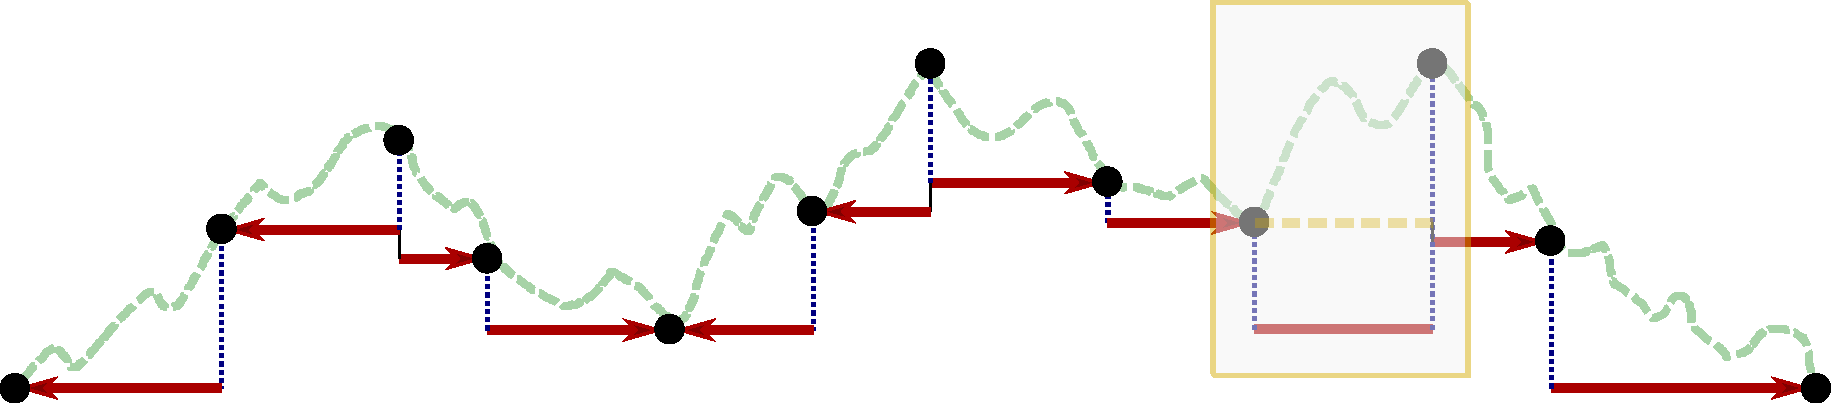
\includegraphics[width=1.0\linewidth, trim={0 12cm 0 12cm}]{images/dyck_boundary_invariant.pdf}
    \caption{Error in third segment.}
    \label{fig:dyck_boundary_invariant}
\end{figure}

It is not even clear that this is always possible.
After sampling the height of a particular position $x_i$ as $h_i$ (with $x_{i-1} < x_i < x_{i+1}$),
the invariant is potentially broken on either side of $x_i$.
We will re-establish the invariant by sampling an additional point on either side.
This proceeds as follows for the interval between $x_i$ and $x_{i+1}$
(see error in Figure~\ref{fig:dyck_boundary_invariant}):
\begin{enumerate}
    \item Sample the lowest height $h$ achieved by the walk between $x_i$ and $x_{i+1}$.
    \item Sample a position $x$ such that $x_i < x < x_{i+1}$ and $\func{Height}(x) = h$.
\end{enumerate}
Since $h$ is the minimum height along this interval, sampling the point $x$ suffices to preserve the invariant.


\subsubsection{Sampling the Lowest Achievable Height}%
\label{ssub:sampling_the_lowest_achievable_height}
For the first step, we need to sample the lowest height of the walk between $x_i$ and $x_{i+1}$.
Notice that we can assume $x_i < x_{i+1}$ without loss of generality (if $x_i > x_{i+1}$, swap them and proceed).
Let's say that the boundary is currently $k'-1$ units below $h_i$.

We know how to count the numnber of possible Dyck paths for any given boundary.
Dividing by the total number of possible paths gives us precisely the CDF we need.
This allows us to binary search to find the boundary.

We will use $D_{k}$ to denote the number of paths that respect a boundary which is $k-1$ units below $h_i$.
So, in the first step, we compute $p = D_{k'/2}/D_{k'}$.
This means that with probability $p$, the path never reaches height $h_i - k'/2$.
Otherwise, the path must reach $h_i-k'/2$ but not $h_i-k'$.
Note that we can also calculate the total number of such paths as $D_{k'} - D_{k'/2}$.
We repeat this procedure, essentially performing binary search,
until we find a $k$ such that the path reaches height $h_i-k+1$ (potentially multiple times), but never goes below it.


\subsubsection{Sampling the Position of First Return}%
\label{sec:sampling_the_location_of_first_return}
Now that we have a ``\emph{mandatory boundary}'' $k$, we just need to sample a position $x$ with height $h = x_i-k+1$.
In fact, we will do something stronger by sampling the \emph{first} time the walk touches the boundary after $x_i$.
\begin{figure}[htpb]
    \centering
    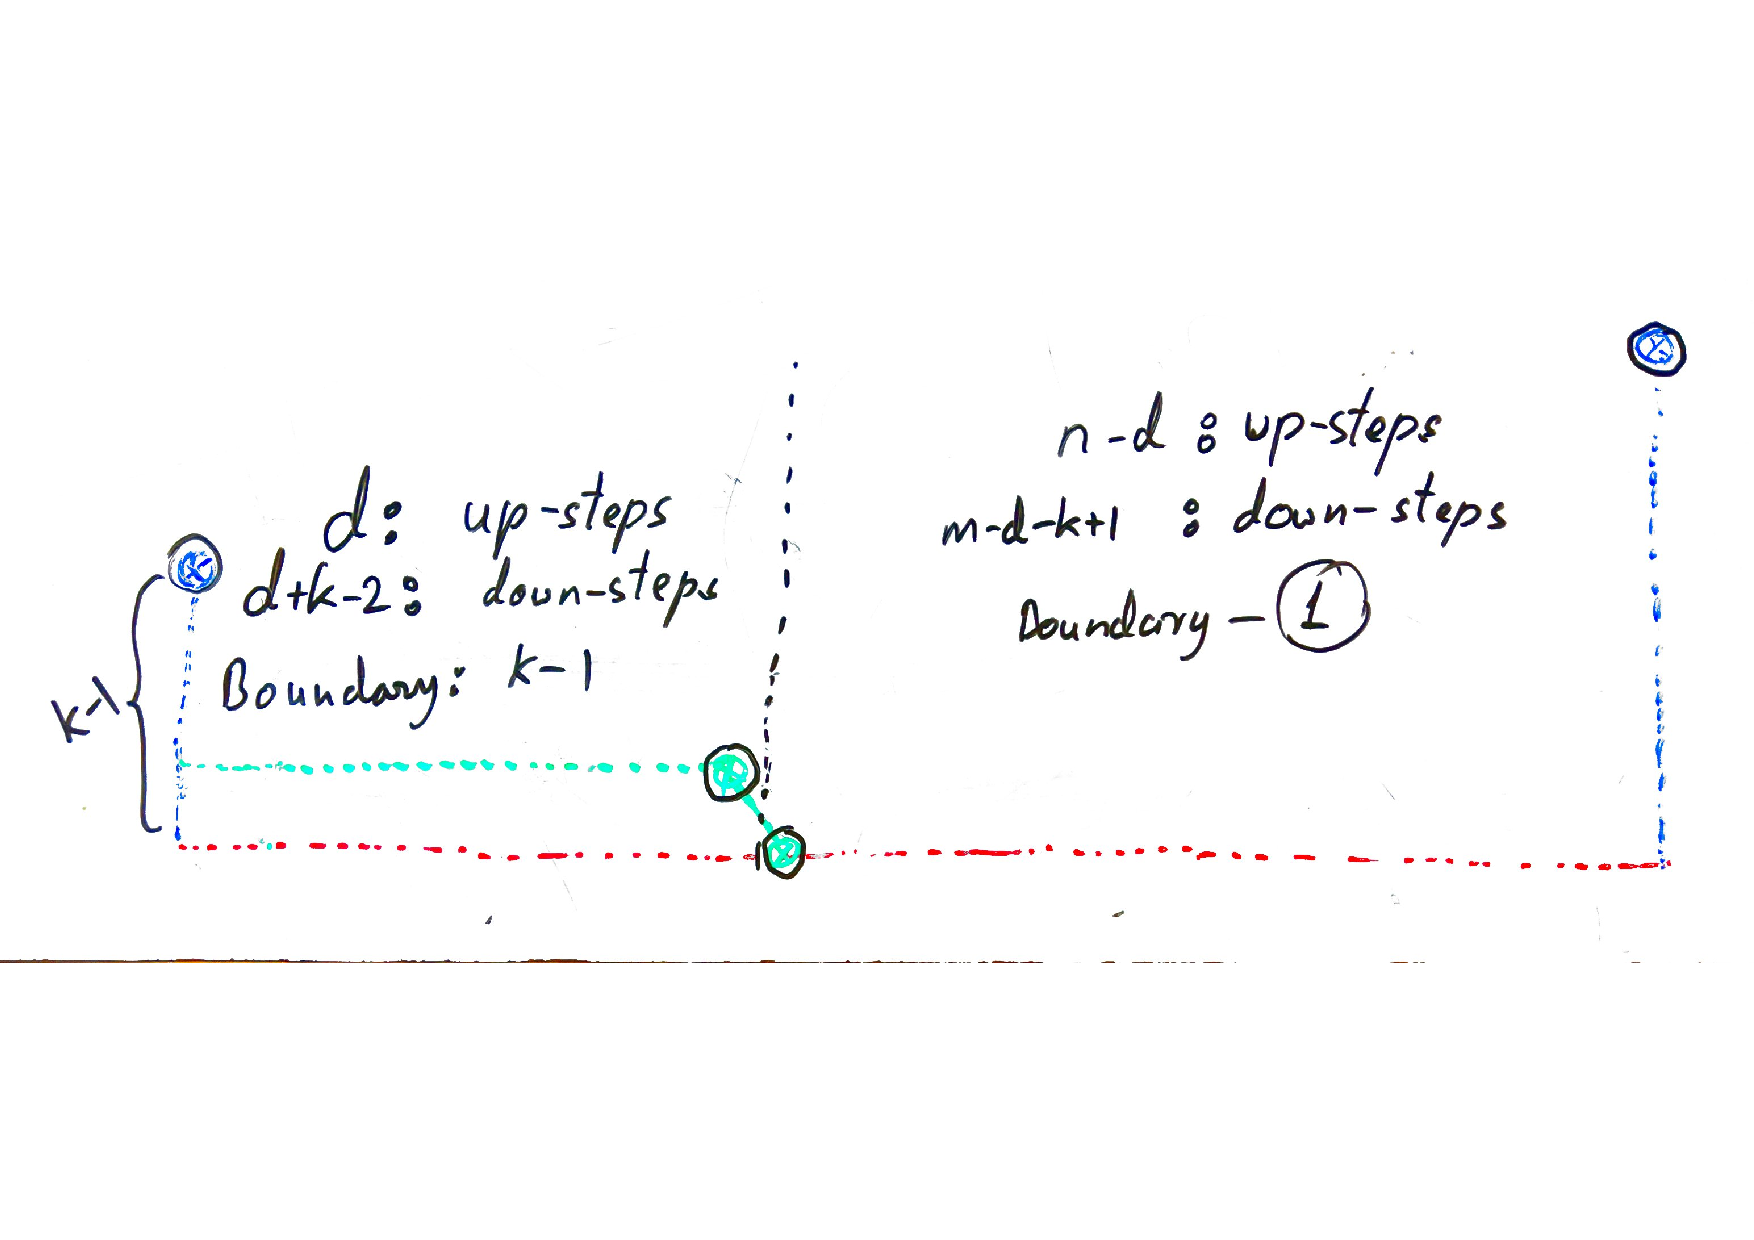
\includegraphics[width=1.0\linewidth, trim={0 6cm 0 5cm}]{images/dyck_return_sampling.pdf}
    \caption{Zooming into (and flipping) the error in Figure~\ref{fig:dyck_return_sampling}}
    \label{fig:dyck_return_sampling}
\end{figure}

We will parameterize the position $x$ the number of up-steps between $x_i$ and $x$
(See Figure~\ref{fig:dyck_return_sampling}).
This quantity will be referred to as $d$ such that $x - x_{i+1} = 2d + k-1$.
Given a specific $d$, we want to compute the number of valid paths that result in
$d$ up-steps before the first approach to the boundary.
We will calculate this quantity by counting the total number of paths to the left and right
of the first approach and multiplying them together.

Since we only care about getting a asymptotic (up to $\poly(\log n)$ factors) estimate of the probabilities,
it suffices to estimate the number of paths asymptotically as well.

\begin{restatable}{lemma}{ReturnDLeftBound}
\label{lem:ReturnDLeftBound}
$D_{left}(d) = \Theta\left( \frac{2^{2d+k}}{\sqrt{d}}\mathlarger e^{-r_{left}(d)}\cdot \frac{k-1}{d+k-1}\right)$
where $r_{left}(d) = \frac{(k-2)^2}{8(2d+k-2)}$.
\end{restatable}

\begin{restatable}{lemma}{ReturnDRightBound}
\label{lem:ReturnDRightBound}
$D_{right}(d) = \Theta\left( \frac{2^{n+m-2d-k}}{\sqrt{n}}\mathlarger e^{-r_{right}(d)}\cdot \frac{n-m+k}{n-d+1}\right)$
where $r_{right}(d) = \frac{(n-m-k-1)^2}{8(n+m-2d-k+1)}$.
\end{restatable}


\subsubsection{Estimating the CDF}%
\label{ssub:estimating_the_cdf}

\begin{restatable}{lemma}{ReturnProbabilityBoundNotNormalized}
\label{lem:ReturnProbabilityBoundNotNormalized}
$D_{left}(d)\cdot D_{right}(d)
= \Theta\left( \frac{2^{n+m}}{dn}\mathlarger e^{-r(d)}\cdot\frac{k-1}{d+k-1}\cdot\frac{n-m+k}{n-d+1}\right)$
where $r(d)=\mathcal O(\log^2 n)$.
\end{restatable}
\begin{proof}
This follows from the fact that both $r_{left}(d)$ and $r_{right}(d)$ are $\mathcal O(\log^2 n)$.
\end{proof}

\begin{corollary}
\label{cor:ReturnProbabilityRounding}
The probability $p_d$ of sampling $d$ as the number of up-steps
before the first approach to the boundary can be approximated as:
\[
p_d = \Theta\left( \frac{ 2^{n+m}\cdot\frac{(k-1)(n-m+k)}{dn(d+k-1)(n-d+1)}\cdot
\mathlarger e^{-\floor{r(d)}} }{\binom{n+m}{n}-\binom{n+m}{m-k}} \right)
\]
\todo{$D_{total}$ is not correct}
This is because the floor function only affects the value of the exponential by a factor of at most $e$.
\end{corollary}
\begin{corollary}
\label{cor:ReturnProbabilityPiecewiseContinuous}
We define a piecewise continuous function
\[
\hat q(d) = \frac{ 2^{n+m}\cdot\frac{(k-1)(n-m+k)}{dn(d+k-1)(n-d+1)}\cdot
\mathlarger e^{-\floor{r(d)}} }{\binom{n+m}{n}-\binom{n+m}{m-k}}
\]
We claim that $p_d = \Theta\left( \int\limits_d^{d+1} \hat q(d)\right)$.
Note that this integral has a closed form for a fixed value of $\floor{r(d)}$.
\end{corollary}


Let the maximum value of $r(d)$ be $r_{max} = \mathcal O(\log^2 n)$.
\begin{corollary}
\label{cor:}
We can compute the approximate normalized probabilities
\[
q_d = \frac{\int\limits_d^{d+1} \hat q(d)}{\int\limits_1^{n} \hat q(d)}
\]
such that $p_d = \Theta(q_d)$.
Furthermore, we can also compute the CDF of $q_d$ as:
\[
Q_d = \frac{\int\limits_1^{d+1} \hat q(d)}{\int\limits_1^{n} \hat q(d)}
\]
This allows us to sample from the distribution $q_d$ and use Lemma~\ref{lem:huge} to indirectly sample from $p_d$.
\end{corollary}


